%\chapter{METHODOLOGY} \label{chap:methodology}
\chapter{\MakeUppercase{\ChapterTitleTwo}} \label{chap:methodology}
    %\doublespacing
    \minitoc
    
    %\newpage
\begin{center}
	%\emph{Abstract of chapter \ref{chap:methodology}}
	\emph{Abstract}
\end{center}
    
    This chapter presents a comprehensive methodology for analyzing the spectral and variability characteristics of Supersoft X-ray Sources (SSS). The spectral analysis section delves into the fundamentals of spectral curve fitting, including model-based fitting, the $\chi^2$ statistic, and parameter estimation. The essential components and data preprocessing steps involved in spectral analysis are also outlined. The variability study section focuses on the application of the Lomb-Scargle periodogram for identifying and characterizing periodic signals within SSS lightcurves. The methodology includes data acquisition, preprocessing, periodogram calculation, statistical significance assessment, phase-folding, and sinusoidal fitting. By combining these techniques, this chapter provides a robust framework for extracting valuable insights into the spectral and variability properties of SSS.
    
    \setcounter{footnote}{\value{footnotecount}}
    
    \newpage
    \section{\MakeUppercase{Spectral Study of Supersoft X-ray Sources}} \label{methodology:spectral}
    	
    	\subsection{Basics of Spectral Curve Fitting}
    		Spectral curve fitting is a fundamental technique in data analysis, particularly in fields involving spectroscopy. It involves modeling observed spectral data using mathematical functions, often with adjustable parameters, to extract meaningful information about the underlying physical processes.

			\subsubsection{The Spectral Fitting Problem}
				Spectrometers do not directly measure the true spectrum of a source. Instead, they record photon counts in specific instrument channels, which are influenced by the instrument's response function. Mathematically, the observed spectrum $C(I)$ is related to the actual spectrum $f(E)$ through the integral equation (\ref{eqn:obs-spec}).
				\begin{align}
					C(I)=\int_0^\infty{f(E)R(I,E)\diff{E}} \label{eqn:obs-spec}
				\end{align}
				In equation (\ref{eqn:obs-spec}), $R(I,E)$ represents the instrument response function, which describes how photons of different energies are detected and recorded in the instrument channels. Inverting this equation to directly obtain the true spectrum from the observed data can be challenging due to non-uniqueness and instability issues. Therefore, an alternative approach of model selection and fitting is commonly adopted.
			
			\subsubsection{Model-Based Fitting}
				In spectral curve fitting, the initial step involves selecting a suitable model spectrum that can adequately represent the observed data. This model is often described by a set of parameters, and is of the form $f(E,p_1,p_2,p_3,\dots)$. These parameters act as adjustable variables that can be modified to fine-tune the shape and characteristics of the model spectrum.
				
				The process of parameter adjustment involves modifying the values of $p_1,p_2,p_3,\dots$ in an iterative manner to minimize the discrepancy between the model spectrum and the observed data. This is essentially a trial-and-error approach where different combinations of parameter values are explored until a satisfactory fit is achieved. The goal is to find the optimal set of parameters that produces a model spectrum that closely aligns with the observed data, capturing the underlying physical processes or phenomena.
			
			\subsubsection{Fitting Methodology}
				Once a suitable model spectrum is chosen and its parameters are defined, the next step involves calculating a predicted count spectrum, denoted as $C_P(I)$. This predicted spectrum is generated by applying the chosen model to the instrument response function and integrating over the energy range. The resulting $C_P(I)$ represents the expected count spectrum based on the model and the instrument's characteristics.

To assess the agreement between the predicted count spectrum and the observed data, a statistical metric known as the fit statistic is employed. The $\chi^2$ statistic is a commonly used fit statistic, which quantifies the deviation between the two spectra. It is calculated as the sum of the squared differences between the observed and predicted counts, normalized by the variance of the observed counts:
				\begin{align}
					\chi^2\equiv\sum{\dfrac{[C(I)-C_P(I)]^2}{(\sigma(I))^2}} \label{eqn:chi-sq}
				\end{align}
				where $C(I)$ is the observed count in channel $I$, $C_P(I)$ is the predicted count in channel $I$, and $\sigma(I)$ is the estimated error in channel $I$. The error term is often approximated as the square root of the observed count, assuming Poisson statistics.
				
				The goal of spectral curve fitting is to find the set of model parameters that minimizes the $\chi^2$ value. This indicates a better agreement between the predicted and observed spectra, suggesting that the chosen model and its parameters accurately describe the underlying physical processes. To achieve this, the parameters are systematically varied and the corresponding $\chi^2$ values are calculated. The set of parameters that yields the lowest $\chi^2$ value is considered the best fit. This iterative process continues until a satisfactory minimum $\chi^2$ value is reached.
			
			\subsubsection{Assessing the Goodness of Fit}
				The reduced $\chi^2$ statistic, defined as:
				\begin{align}
					\chi^2_\text{red}=\dfrac{\chi^2}{\nu} \label{eqn:chisq-reduced}
				\end{align}
				provides a valuable metric for evaluating the quality of the fit between a model and the observed data. Here, $\nu$ is the degrees of freedom, which is calculated as the difference between the number of channels and the number of model parameters. This effectively accounts for the constraints imposed by the model on the data.
				
				The $\chi^2_\text{red}$, as a fit statistic, may be used to assess the goodness of the fit as follows:
				\begin{itemize}
					\item \textit{Good Fit}: When the $\chi^2_\text{red}$ value is close to 1, it indicates a satisfactory agreement between the model and the data. This suggests that the model captures the underlying physical processes effectively and that the estimated errors are reasonable.
					\item \textit{Poor Fit}: A $\chi^2_\text{red}$ value significantly greater than 1 suggests a poor fit. This could be due to several factors, such as an inadequate model, underestimated errors, or systematic biases in the data. A poor fit may necessitate revisiting the model choice or refining the error estimation.
					\item \textit{Overestimated Errors}: A $\chi^2_\text{red}$ value significantly less than 1 indicates that the errors on the data have been overestimated. This could be attributed to various factors, including underestimation of systematic uncertainties or the presence of correlations between data points.
				\end{itemize}
				
				The $\chi^2_\text{red}$ statistic provides a quantitative measure of the goodness-of-fit. It allows for a systematic comparison of different models and helps identify potential shortcomings or inconsistencies in the data or the chosen model. By analyzing the deviation of the $\chi^2_\text{red}$ value from 1, one can gain insights into the quality of the fit and make informed decisions regarding the suitability of the model and the reliability of the extracted information.
			
			\subsubsection{Error Estimation}
				The error width, which quantifies the uncertainty associated with the estimated parameters in spectral curve fitting, can be derived from the covariance matrix obtained during the fitting process. The covariance matrix is a square matrix that provides information about the relationships between the parameters and their associated uncertainties.
				
				The diagonal elements of the covariance matrix represent the variances of the individual parameters. The square root of the diagonal elements gives the standard deviations, which can be interpreted as the error widths. These standard deviations indicate the range of values within which the true parameter value is likely to lie with a certain level of confidence.
				
				The off-diagonal elements of the covariance matrix represent the covariances between pairs of parameters. These values indicate the degree of correlation between the uncertainties in the parameters. A high covariance between two parameters suggests that their uncertainties are interrelated, meaning that changes in one parameter may affect the uncertainty in the other. By examining the covariance matrix, it is possible to identify potential correlations between parameters and assess their impact on the overall uncertainty in the fitted model.
			
    	\subsection{Software Implementation}
    		
    		\subsubsection{Essential Components}
    			Any generic software implementation of spectral curve fitting necessitates the presence of the following essential components for modeling and interpreting observed spectral data:
    			\begin{enumerate}
    				\item \textit{Observed Spectra} $D(I)$: The core component of spectral curve fitting is the observed spectral data, denoted as $D(I)$. This dataset represents the measured intensity of radiation as a function of detector channels $I$. The detector channels correspond to specific energy ranges or wavelengths, capturing the spectral information of the observed phenomenon.
    				\item \textit{Background Measurements} $B(I)$: In most practical scenarios, the observed spectra are contaminated by background radiation or noise. To accurately isolate the signal of interest, background measurements, denoted as $B(I)$, are typically acquired. These measurements represent the instrumental background signal in the absence of the target source. By subtracting the background measurements from the observed spectra, it is possible to remove the unwanted noise and isolate the signal of interest.
    				\item \textit{Instrument Response} $R(I,E)$: The instrument response function $R(I,E)$ maps the detector channels to the corresponding energy bins, providing a relationship between the observed spectral data and the underlying physical phenomenon. The instrument response function accounts for the instrument's sensitivity, resolution, and other characteristics, enabling the accurate interpretation of the measured spectral data.
    				\item \textit{Model Spectra} $M(E)$: A set of model spectra $M(E)$ represent a variety of potential spectral shapes based on different physical scenarios or theoretical models. By comparing the observed spectra to these model spectra, one can identify the most suitable model and extract valuable information about the underlying physical processes. The choice of model spectra depends on the specific application and the expected characteristics of the observed phenomenon.
    			\end{enumerate}
    		
    		\subsubsection{Data Processing and Model Construction}
    			\paragraph{Background subtraction:}
    			The observed spectrum $C(I)$ is typically contaminated by background radiation or noise. To isolate the signal of interest, the background spectrum $B(I)$ is subtracted from the raw data. This process is represented by equation (\ref{eqn:spec-backsub}) as given below:
    			\begin{equation}
					C(I)=\dfrac{D(I)}{a_Dt_D}-\dfrac{b_D}{b_B}\dfrac{B(I)}{a_B t_B} \label{eqn:spec-backsub}
				\end{equation}
				where the following scaling factors and exposure times are used to normalize the spectra and ensure accurate background subtraction:
				\begin{itemize}
					\item $a_D,a_B$: Area scaling factors to account for differences in the area of the detector or source regions
					\item $b_D,b_B$: Background scaling factors to adjust the relative contribution of the background
					\item $t_D,t_B$: Exposure times for the observed data and background measurements, respectively
				\end{itemize}
				
				\paragraph{Instrument response function:}
				The instrument response function $R(I,E)$ maps the detector channels to the corresponding energy bins. It characterizes how the instrument responds to different energies. The instrument response function is typically a continuous function that can be discretized for computational efficiency. In order to do so, the energy range is divided into bins $E_j$. The corresponding response matrix elements $R_D(I,j)$ are calculated by integrating the continuous function $R(I,E)$ over each energy bin as given in equation (\ref{eqn:spec-response}):
				\begin{equation}
					R_D(I,j)=\dfrac{1}{E_j-E_{j-1}}{\int_{E_{j-1}}^{E_j}{R(I,E)\diff{E}}} \label{eqn:spec-response}
				\end{equation}
				This discretization process transforms the continuous function into a matrix, which is suited for numerical calculations.
				
				\paragraph{Auxiliary response function:}
				In some cases, additional effects such as energy redistribution within the detector can be accounted for by introducing an auxiliary response function $A_D(j)$. This function modifies the instrument response matrix elements as follows:
				\begin{equation*}
					R_D(I,j)\quad\rightarrow\quad R_D(I,j)\cdot A_D(j)
				\end{equation*}
				The auxiliary response function effectively redistributes the counts between energy bins, capturing the effects of energy-dependent phenomena within the detector. This represents the \textit{redistribution matrix function} (RMF).
				
				\paragraph{Model spectra discretization:}
				Similar to the instrument response function, the model spectra $M(E)$ are also discretized to match the energy bins used for the analysis. This discretization is performed by integrating the model spectra over the corresponding energy bins:
				\begin{equation}
					M_D(j)=\int_{E_{j-1}}^{E_j}{M(E)\diff{E}} \label{eqn:spec-model}
				\end{equation}
				The discretized model spectra $M_D(j)$ can then be used in conjunction with the instrument response matrix and observed data to calculate the predicted count spectrum.

    		
    		\subsubsection{Predicted Spectrum and Fit Statistic}
    			The predicted count spectrum $C_P(I)$ represents the expected counts in each detector channel based on the chosen model and the instrument response. It is calculated by multiplying the instrument response matrix $R_D(I,j)$ with the model spectrum $M_D(j)$ as per equation (eqn:spec-predcounts):
    			\begin{equation}
					C_P(I)=R_D(I,j)\cdot M_D(j) \label{eqn:spec-predcounts}
				\end{equation}
				This matrix multiplication effectively applies the instrument response to the model spectrum, accounting for the detector's sensitivity and energy resolution. The resulting predicted count spectrum provides a theoretical expectation of the observed counts, assuming the model accurately describes the underlying physical processes.
				
				To quantify the agreement between the predicted count spectrum and the observed data, the fit statistic $\chi^2$ is computed in a discretized form as given in equation ():
				\begin{equation}
					\chi^2=\sum_I{[C(I)-C_P(I)]^2} \label{eqn:spec-chisq-software}
				\end{equation}

    		
    		\subsubsection{General Fitting Framework}
    			Spectral curve fitting can be formulated as an optimization problem, where the goal is to find the optimal parameters that minimize an objective function $S$. Such an optimization problem may be stated in general as follows:
    			
    			\begin{quotation}
    				Given a set of spectra $\mathbb{C}(I)$, each supplied as a function of detector channels, a set of theoretical models {$\mathbb{M}(E)_j$}, each expressed in terms of a vector of energies together with a set of functions {$\mathbb{R}(I,E)_j$} that map the channels to the energies, minimize an objective function $S$ of $\mathbb{C}$, {$\mathbb{R}(I,E)_j$}, {$\mathbb{M}(E)_j$} using a fitting algorithm. The objective function $S$ may be expressed as per equation ():
    				\begin{align}
						S=S(\mathbb{C},\sum_k{\mathbb{M}_j^k\cdot\mathbb{R}_j^k}) \label{eqn:spec-gen-framework}
					\end{align}
    			\end{quotation}
    			
    			In the context of the spectral fitting of SSS, the objective function which is to be optimized is the $\chi^2$ statistic. The \textit{Levenberg-Marquardt algorithm} is a widely used optimization technique for minimizing the $\chi^2$ statistic. It combines the features of the steepest descent and Gauss-Newton methods, providing a robust and efficient approach to finding the optimal parameter values.
    			
    			The Levenberg-Marquardt algorithm iteratively updates the parameter values based on the gradient of the $\chi^2$ function and a damping parameter $\lambda$. The damping parameter controls the balance between the steepest descent and Gauss-Newton methods, allowing the algorithm to adapt to different optimization landscapes. By iteratively adjusting the parameters and evaluating the $\chi^2$ statistic, the Levenberg-Marquardt algorithm effectively finds the parameter values that minimize the objective function and yield the best fit between the model and the observed data.

		\subsection{Implementation of Spectral Fitting Using XSPEC}
			Here we outline the methodology employed for the spectral analysis of SSS using the XSPEC software \cite{xspecManualv12_9_1}. The analysis involves fitting spectral models to data extracted from various X-ray observatories to determine the physical properties of these sources. By following these steps, the spectral analysis of SSS can provide valuable insights into their physical properties, including effective temperatures, column densities, and the presence of elemental absorption features.
			
			\subsubsection{Data Reduction and Model Selection}
				\begin{enumerate}[I.]
					\item A grid of viable spectral models is established to explore different physical scenarios and potential fits to the data.
					\item The raw event files are processed to extract four (or three) FITS files:
					\begin{enumerate}[i.]
						\item the source spectrum
						\item the background spectrum
						\item the response matrix file
						\item the auxiliary response file (if available).
					\end{enumerate}
					\item The extracted FITS files are combined into a spectral group using the \texttt{grppha} command, specifying the minimum bin size for the spectral data.
				\end{enumerate}
			
			\subsubsection{Spectral Analysis in XSPEC}
				\begin{enumerate}[I.]
					\item The grouped data is loaded into XSPEC using the \texttt{data} command. The \texttt{cpd} command opens the plotting window, and the \texttt{plot} command displays the spectrum, allowing for visual inspection and identification of potential issues.
					\item Bad channels and energy bins outside the region of interest are excluded using the \texttt{ignore} command.
					\item A multi-component model is defined in XSPEC using the \texttt{model} command. This model can include additive and multiplicative components to represent various physical processes.
					\item For non-local thermodynamic equilibrium (NLTE) components, the \texttt{atable} command is used to incorporate appropriate table models.
					\item Elemental abundances and initial values for model parameters are set based on prior knowledge or literature values.
					\item The \texttt{renorm} command is used to renormalize the model, and the \texttt{fit} command is employed to fit the model to the grouped spectral data.
				\end{enumerate}
			
			\subsubsection{Model Evaluation and Parameter Estimation}
				\begin{enumerate}[I.]
					\item The $\chi^2$ statistic and degrees of freedom are examined to calculate the reduced $\chi^2$ value. Visual inspection of the data, model, residuals, and delchi values helps assess the suitability of the model fit.
					\item If necessary, the model parameters are iteratively modified using manual adjustments or the \texttt{steppar} command to achieve the best possible fit. Different models from the grid may be explored if the initial fit is unsatisfactory.
					\item The plot data is saved to ASCII files using the \texttt{WData} command of QDP-PLT by extracting directly from the plot window.
				\end{enumerate}
			
			\subsubsection{Result Reporting and Analysis}
				\begin{enumerate}[I.]
					\item The fitting statistic of the best-fit model is reported in tabular format.
					\item The error \texttt{command} is used to calculate the uncertainties in the parameter values. The \texttt{parallel} command can be employed to simultaneously compute error ranges for multiple parameters.
					\item The best-fit values of parameters such as effective temperature and column density, along with their error ranges, are reported.
					\item The absorbed and unabsorbed fluxes are computed using the \texttt{cflux} model component.
					\item The source luminosity is calculated using the unabsorbed flux and the constrained distance to the source, as per the Stefan-Boltzmann law.
					\item The unfolded spectrum is visually inspected to identify the presence of elemental absorption edges. Literature searches are conducted to identify the corresponding elements and their spectral states.
					\item The plot data is saved to ASCII files using the \texttt{WData} command of QDP-PLT by extracting directly from the plot window.
					\item The ASCII files containing the plot data are loaded into Python using NumPy and Matplotlib. Relevant plots are created and analyzed to extract additional insights from the spectral data.
				\end{enumerate}
			

    \section{\MakeUppercase{Variability Study of Supersoft X-ray Sources}} \label{methodology:variability}
    
    	\subsection{Introduction to Lomb-Scargle Periodogram}
    		Periodograms are a versatile tool for identifying and quantifying periodic patterns within data. By transforming a time series into the frequency domain, periodograms reveal the frequencies at which the signal exhibits significant power. This spectral analysis is invaluable for detecting periodic components that might be obscured in the original time domain representation.
    		
    		The height of peaks in a periodogram provides an estimate of the amplitude of the corresponding periodic component. This allows for a quantitative assessment of the strength of periodic signals. Additionally, the frequency of these peaks directly indicates the periodicity of the underlying patterns.
    		
    		While traditional periodograms are well-suited for uniformly sampled data, their applicability can be limited when dealing with irregularly spaced time series. In such scenario, the Lomb-Scargle periodogram emerges as a viable alternative \cite{lomb1976least,scargle1982studies}. Specifically designed to handle unevenly spaced data, the Lomb-Scargle periodogram accounts for gaps in the time series, providing a robust and reliable method for detecting periodic signals.
    		
    	\subsection{Theory of Lomb-Scargle Periodogram}
    		The Lomb-Scargle periodogram is a robust and versatile technique for analyzing unevenly sampled time series data, particularly prevalent in astronomical applications. This method provides a computationally efficient approach to estimate a Fourier-like power spectrum, enabling the identification and characterization of periodic signals embedded within noisy or irregularly spaced data \cite{vanderplas2018understanding}.
    		
    		By leveraging the Lomb-Scargle algorithm, one can effectively determine the dominant oscillation period of a given time series. The method's ability to handle gaps and variations in sampling intervals makes it indispensable for analyzing astronomical observations, where data collection is often subject to constraints such as weather conditions, instrument limitations, or observational scheduling.
    	
    		\subsubsection{Uniform and Non-uniform Sampling of Data}
    			\paragraph{Uniform sampling of data:}
    			Suppose that $g(t)$ is a \textit{signal function} and $W(t)$ represents the observation \textit{window function}, then the observed signal is represented by the following function:
    			\begin{align}
    				g_\text{obs}(t)=g(t)W(t) \label{eqn:obs-func}
    			\end{align}
    			Then, by the Fourier convolution theorem, we have,
    			\begin{align}
    				\mathscr{F}\left\lbrace g_\text{obs} \right\rbrace = \mathscr{F}\left\lbrace g(t) \right\rbrace * \mathscr{F}\left\lbrace W(t) \right\rbrace \label{eqn:FT-obs-func}
    			\end{align}
    			In the case of the discrete Fourier transform, where the continuous signal is sampled at regular intervals, the window function becomes a Dirac comb, which is a regular grid of Dirac delta functions with spacing of $\Delta t$, i.e.
    			\begin{align}
    				W(t)=\text{III}_{\Delta t}(t)=\sum_{n=-\infty}^{\infty}{\delta(t-n\Delta t)} \label{eqn:dirac-comb}
    			\end{align}
    			
    			Hence, equation \ref{eqn:obs-func} becomes
    			\begin{align}
    				g_\text{obs}(t)=g(t)\text{III}_{\Delta t}(t) \label{eqn:obs-func:dft}
    			\end{align}
    			Taking the Fourier transform of equation (\ref{eqn:obs-func:dft}), we can have
    			\begin{align}
    				\hat{g}_\text{obs}(f)&=\FT{g_\text{obs}(t)}{f} \nonumber \\
    					&=\FT{g(t)\text{III}_{\Delta t}(t)}{f} \nonumber \\
    					&=\FT{g(t)\left\lbrace \sum_{n=-\infty}^{\infty}{\delta(t-n\Delta t)} \right\rbrace}{f} \nonumber \\
    					&=\sum_{n=-\infty}^{\infty}{\int_{-\infty}^{\infty}{\delta(t-n\Delta t)g(t)e^{-2\pi ift}\diff{t}}} \nonumber \\
    				\implies\hat{g}_\text{obs}(f)&=\sum_{n=-\infty}^{\infty}{g(n\Delta t)e^{-2\pi ift}} \label{eqn:dft-01}
    			\end{align}
    			In case of a finite number $N$ of samples, we can express $g(n\Delta t)=g_n$ and so equation (\ref{eqn:dft-01}) becomes
    			\begin{align}
    				\hat{g}_\text{obs}(f)&=\sum_{n=0}^{N}{g_ne^{-2\pi ifn\Delta t}} \label{eqn:dft-02}
    			\end{align}
    			As per the Nyquist limit, the frequency range of relevance is $0\leqslant f\leqslant\dfrac{1}{\Delta t}$. This range can be evenly spaced into $N$ intervals with
    			\begin{align*}
    				\Delta f&=\dfrac{1/{\Delta t}}{N}=\dfrac{1}{N\Delta t} \\
    				\implies\Delta f\Delta t&=\dfrac{1}{N}
    			\end{align*}
    			Let the frequency range be spaced by $\Delta f$, i.e. $f=k\Delta f$, where $k$ is an integer. Then from equation (\ref{eqn:dft-02}), we obtain
    			\begin{align}
    				\hat{g}_\text{obs}(k\Delta f)&=\sum_{n=0}^{N}{g_ne^{-2\pi ik\Delta fn\Delta t}} \nonumber \\
    				\implies \hat{g}_k&=\sum_{n=0}^{N}{g_ne^{-2\pi ikn/N}} \label{eqn:dft-03}
    			\end{align}
    			Here, equation (\ref{eqn:dft-03}) gives the expression for the implementation of the discrete Fourier transform.
    			
    			From the DFT in equation (\ref{eqn:dft-03}), we can compute the \textit{classical periodogram} or \textit{Schuster periodogram} \cite{schuster1898investigation} as $\dfrac{1}{N}$ times the Fourier power spectrum for a continuous signal observed with uniform sampling using a Dirac comb:
    			\begin{align}
    				P_s(f)=\dfrac{1}{N}\left| \sum_{n=1}^{N}{g_ne^{-2\pi i ft_n}} \right|^2 \label{eqn:schuster-periodogram}
    			\end{align}
    			It must be clarified here that the periodogram is a statistic which is computed from the data and it is used to estimate the power spectrum of the underlying continuous signal of interest.
    			
    			In real-world observational fields such as astronomy, data collection is often subjected to a range of constraints and variability, leading to non-uniform sampling. Unlike controlled experiments where conditions can be held constant, astronomical observations by space-based observatories are influenced by a variety of factors:
    			\begin{enumerate}[i.]
    				\item \textit{Orbital constraints}: Space-based telescopes are often in specific orbits around the Earth, the Moon, or even the Sun. These orbits dictate observation windows and create periods when the telescope cannot point at certain objects due to the Sun, Earth, or other celestial bodies obstructing the line of sight.
    				\item \textit{Sun avoidance regions}: To prevent damage to sensitive instruments, space-based telescopes typically have sun avoidance zones where they cannot observe. This limits the ability to track certain objects continuously, leading to gaps in data collection.
    				\item \textit{Limited data storage and downlink bandwidth}: Space telescopes have finite onboard data storage and are dependent on ground stations for data downlink. Periods when the telescope is out of communication range or when storage reaches capacity can result in interruptions in data collection.
    				\item \textit{Thermal constraints and cooling periods}: Space-based telescopes equipped with infrared sensors or other heat-sensitive instruments may require cooling periods or specific thermal management strategies. This can restrict observation times and introduce non-uniform sampling in the data.
    				\item \textit{Instrument maintenance and calibration}: Routine instrument calibration and maintenance activities can lead to temporary suspension of scientific observations, causing gaps in data collection.
    			\end{enumerate}
    			These factors create unevenly spaced data points that pose significant challenges for the discrete Fourier transform, which is built on the assumption of uniform sampling intervals.
    			
    			\paragraph{Non-uniform sampling of data:}
    			In case the observed data is a signal that is sampled over a set of $N$ times, i.e. $\{t_n\}$, and so the window function my be expressed as
    			\begin{align}
    				W_{\{t_n\}}(t)=\sum_{n=1}^{N}{\delta(t-t_n)} \label{eqn:nonunif-dirac-comb}
    			\end{align}
    			In this scenario, upon applying the window function to the underlying continuous signal, the observed signal is obtained to be of the form:
    			\begin{align}
    				g_\text{obs}(t)&=g(t)W_{\{t_n\}}(t) \nonumber \\
    				\implies g_\text{obs}(t)&=\sum_{n=1}^{N}{g(t)\delta(t-t_n)} \label{eqn:obs-func-nonunif}
    			\end{align}
    			The Fourier transform of the observed signal is obtained using the convolution theorem to be as follows
    			\begin{align}
    				\mathscr{F}\{g_\text{obs}\}=\mathscr{F}\{g(t)\}*\mathscr{F}\{W_{\{t_n\}}(t)\} \label{eqn:FT-obs-func-nonunif}
    			\end{align}
    			However, in this case, the Fourier transform of the window function $W_{\{t_n\}}(t)$ would not be a Dirac comb. Rather, it would be noisier because the observation times have undergone randomization. Even though this noise may be reduced to a certain degree by increasing the number of observations, it would still persist. Also, increasing the number of observations might not be practically feasible in situation, such as in astronomy.
    				
    		\subsubsection{Mathematical Formulation of Lomb-Scargle Periodogram}
    			Using Euler's formula, the classical periodogram given in equation (\ref{eqn:schuster-periodogram}) can be re-cast in the following manner:
    			\begin{align}
    				P(f)&=\dfrac{1}{N}\left| \sum_{n=1}^{N}{g_ne^{-2\pi i ft_n}} \right|^2 \nonumber \\
    				\implies P(f)&=\dfrac{1}{N}\left[ \left\lbrace \sum_{n=1}^{N}{g_n\cos{(2\pi ft_n)}} \right\rbrace^2 + \left\lbrace \sum_{n=1}^{N}{g_n\sin{(2\pi ft_n)}} \right\rbrace^2 \right] \label{eqn:lomb-scargle-01}
    			\end{align}

    			When the classical periodogram is applied to uniformly-sampled Gaussian noise, its distribution converges asymptotically to a $\chi^2$ distribution with known degrees of freedom, this property being contingent upon the assumption of uniform sampling. For non-uniformly sampled data, the distribution of the periodogram becomes considerably more complex, and a closed-form analytical expression is generally intractable.
    			
    			To address this issue, Scargle generalized the periodogram in equation (\ref{eqn:lomb-scargle-01}) as follows \cite{scargle1982studies}:
    			\begin{align}
    				P(f)&=\dfrac{A^2}{2}\left\lbrace \sum_{n=1}^{N}{g_n\cos{[2\pi f(t_n-\tau)]}} \right\rbrace^2 + \dfrac{B^2}{2}\left\lbrace \sum_{n=1}^{N}{g_n\sin{[2\pi f(t_n-\tau)]}} \right\rbrace^2 \label{eqn:lomb-scargle-02}
    			\end{align}
    			where $A$, $B$ and $\tau$ are arbitrary functions of the frequencies $f$ and the observing times $\{t_i\}$. Scargle also showed that one can choose unique forms of $A$, $B$ and $\tau$ in a manner such that we have the periodogram in equation (\ref{eqn:lomb-scargle-02})
    			\begin{enumerate}[a)]
    				\item reducing to the classical form in equation (\ref{eqn:schuster-periodogram}) in case the observations are uniformly sampled.
    				\item having statistics which are analytically computable.
    				\item becoming insensitive to global time-shifts in data.
    			\end{enumerate}
    			The functions of $A$, $B$ and $\tau$ that provide the above properties are
    			\begin{align*}
    				A&=\dfrac{1}{\sqrt{\sum_{n}{\cos^2{[2\pi f(t_n-\tau)]}}}} \\
    				B&=\dfrac{1}{\sqrt{\sum_{n}{\sin^2{[2\pi f(t_n-\tau)]}}}} \\
    				\tau&=\dfrac{1}{4\pi f}\tan^{-1}{\left\lbrace \dfrac{\sum_{n}{\sin{[4\pi ft_n)]}}}{\sum_{n}{\cos{[4\pi ft_n)]}}} \right\rbrace}
    			\end{align*}
    			In the above, the function $\tau$ ensures the time-shift invariance of the Lomb-Scargle periodogram. A notable feature of the Lomb-Scargle periodogram is its equivalence to the result obtained from fitting a simple sinusoidal model to the data at each frequency $f$ and constructing a periodogram from the $\chi^2$ goodness-of-fit statistic at each frequency. This approach allows the periodogram to be viewed as a measure of how well a sine wave of a given frequency fits the observational data. In this context, the introduction of the $\tau$ shift is crucial, as it serves to orthogonalize the normal equations used in the least squares fitting process. This orthogonalization ensures that the fitting procedure is unbiased and more computationally stable. This deep connection between traditional Fourier analysis and least-squares analysis has led to the widespread adoption of the term \textit{Lomb-Scargle periodogram} to describe this methodology, even though variants of this approach were utilized prior to Lomb and Scargle's formalization.
    			
    		\subsubsection{Units in the Lomb-Scargle Periodogram}
    			From a given time-series data array, the computed Lomb-Scargle periodogram, from equation (\ref{eqn:lomb-scargle-02}), can be visualized as a two-dimensional plot. The horizontal axis represents the range of periods that were tested in the analysis. It is essentially a grid of potential periods that the Lomb-Scargle algorithm evaluates to determine the likelihood of a periodic signal at that particular period.
    			
    			The vertical axis represents the power associated with each period. It is a measure of how well the periodic signal fits the data at that particular period. Higher power values indicate a stronger likelihood of a periodic signal at that period. The power values in the Lomb-Scargle periodogram are dimensionless. They are calculated based on the correlation between the data and a sinusoidal model at each period, and the units cancel out during the calculations.
    			
    		\subsubsection{Uncertainties in Periodogram Results}
    			A critical aspect of reporting results derived from the Lomb-Scargle periodogram is the quantification of uncertainty associated with the estimated period. While traditional approaches often rely on error bars to express uncertainty, such a metric may be less meaningful in the context of Lomb-Scargle periodograms. The primary concern with periodograms is often the presence of false peaks or aliases, rather than a continuous distribution of potential period values around a true estimate. This disjointed nature of uncertainty necessitates a more nuanced approach to quantifying the reliability of the estimated period.
    			
    			\paragraph{Peak width and frequency precision:}
    			The presence of a peak within the Lomb-Scargle periodogram, characterized by its width and height, signifies the existence of a periodic signal. In the Fourier domain, the precision with which a peak's frequency can be identified is directly correlated with its width. A common metric for quantifying this width is the half-width at half-maximum, denoted by $f_{1/2}\approx T$.
    			
    			A more rigorous framework for assessing uncertainty can be established within the context of least squares analysis. In this interpretation, the inverse of the peak's curvature is directly related to the uncertainty in the estimated frequency. This perspective aligns with the Bayesian approach, which involves fitting a Gaussian curve to the exponentiated peak. The Bayesian uncertainty in the frequency estimate is influenced by both the number of samples $N$, and the average signal-to-noise ratio $\Sigma$. The scaling of this uncertainty can be approximated by the standard deviation of the estimated frequency:
    			\begin{align}
    				\sigma_f\approx\sqrt{\dfrac{2}{N\Sigma^2}} \label{eqn:stddev-est-freq}
    			\end{align}
    			This dependence arise from the fact that the Bayesian uncertainty is linked to the width of the exponentiated periodogram, which in turn is influenced by the height of the peak $P_\text{max}$.
    			
    			\paragraph{False alarm probability:}
    			A more pertinent metric for assessing the uncertainty associated with Lomb-Scargle periodogram results is the relative height of the signal peak to the background noise. The spurious peaks that arise in the periodogram are influenced by both the sample size $N$, and the signal-to-noise ratio. For scenarios with limited data and low signal-to-noise, these spurious peaks can rival the height of the true signal peak, making it challenging to distinguish between genuine and chance-driven features.
    			
    			The False Alarm Probability (FAP) serves as a standard approach for quantifying the significance of a periodogram peak. It represents the probability that a dataset devoid of any true signal would, due to random fluctuations in the noise, produce a peak of comparable magnitude. Scargle (1982) demonstrated that for pure Gaussian noise at any given frequency $f_0$, the unnormalized Lomb-Scargle periodogram statistic $Z=P(f_0)$, follows a $\chi^2$ distribution with two degrees of freedom. Consequently, the cumulative probability of observing a periodogram value less than $Z$ can be expressed as:
    			\begin{align}
    				P_\text{single}(Z)=1-\exp(-Z) \label{eqn:L-S-fap-01}
    			\end{align}
    			Equation (\ref{eqn:L-S-fap-01}) provides a quantitative measure of the likelihood that a given peak is due to chance.
    			
    			The FAP measures the likelihood that a peak in the periodogram is due to chance, rather than a genuine periodic signal. A low FAP means that the observed peak is unlikely to be a false alarm. Therefore, for a periodic signal to be considered significant, the corresponding FAP should be small. This suggests that the peak is highly likely to represent a real periodic component within the data.
    			
    			\paragraph{The Baluev method:}
    			Baluev (2008) \cite{baluev2008assessing} introduced a refined approximation for the False Alarm Probability (FAP) in the context of Lomb-Scargle periodograms. This approximation, given by:
    			\begin{align}
    				\text{FAP}(z)\approx 1 - P_\text{single}(z)e^{-\tau(z)}\label{eqn:L-S-fap-baluev-01}
    			\end{align}
    			provides a conservative upper bound, even for time series characterized by highly structured window functions. Here, $P_\text{single}$ denotes the cumulative probability of observing a periodogram value less than $Z$ under the null hypothesis, while $\tau(z)$ is a correction factor defined as $\tau(z)\approx W(1 - z)^{(N-4)/2}\sqrt{z}$, where $W$ represents the effective width of the observing window in units of the maximum frequency and $N$ is the total number of data points.
    			
    			While this approximation is not exact, it offers a reliable upper bound for alias-free periodograms. Notably, it maintains a reasonable degree of accuracy even for more realistic survey windows that exhibit non-trivial structure. The Baluev method has become the standard algorithm for computing the FAP in many software implementations of the Lomb-Scargle periodogram.
    		
    	\subsection{Implementation of Lomb-Scargle Periodogram}
    		Here we outline the methodology we have employed to investigate the variability characteristics of lightcurves extracted from SSS across two energy ranges: 0.2-1.0 keV and 0.2-12.0 keV. The analysis leverages the Lomb-Scargle periodogram to identify and characterize periodic signals within the lightcurves. By systematically applying these steps to the lightcurves of SSS at the two specified energy ranges, this methodology enables a comprehensive characterization of their variability patterns. The combination of Lomb-Scargle periodogram analysis, statistical significance evaluation, phase-folding, and sinusoidal fitting provides a robust framework for uncovering periodic signals and quantifying their properties within the lightcurve data.
    		    	
    		\subsubsection{Data Acquisition and Preprocessing}
    			\begin{enumerate}[I.]
    				\item Google Drive is mounted within Google Colab to facilitate seamless access to the relevant FITS files containing the lightcurve data.
    				\item The \texttt{astropy.io} module's \texttt{fits.open()} function is used to open the FITS files and extract the lightcurve data.
    				\item The extracted lightcurve information is converted into \texttt{NumPy} arrays for efficient numerical operations.
    				\item Visual inspection of the lightcurve is performed to identify potential outliers. These outliers, if present, are removed using \texttt{NumPy} masks to ensure they don't influence the subsequent analysis. The cleaned lightcurve is then visualized.
    			\end{enumerate}
    		
    		\subsubsection{Timing Analysis Using Lomb-Scargle Periodogram}
    			\begin{enumerate}[I.]
    				\item A \texttt{LombScargle} object is created using the \texttt{astropy.timeseries} module. This object encapsulates the time and rate arrays extracted from the lightcurve to compute the Lomb-Scargle periodogram.
    				\item The calculated Lomb-Scargle periodogram is utilized to retrieve the corresponding frequency and power arrays using the \texttt{autopower()} method of the \texttt{LombScargle} object.
    				\item The Lomb-Scargle periodogram is displayed graphically. Prominent peaks are visually identified for further analysis.
    				\item Peaks corresponding to harmonics associated with the observation window and the time bin size are disregarded, as they do not represent genuine periodicities within the lightcurve data. Rather these are artefacts due to the observation cadence and the time binning process.
    			\end{enumerate}
    		
    		\subsubsection{Statistical Significance and Phase-Folded Lightcurves}
    			\begin{enumerate}[I.]
    				\item The \texttt{false\_alarm\_probability()} method of the \texttt{LombScargle} object is employed to compute the FAP for the identified peaks. This metric quantifies the probability of observing such peaks arising purely from random noise.
    				\item Employing the periods corresponding to the identified significant peaks, phase-folded lightcurves are constructed. These lightcurves represent the binned data points as a function of their phase within a complete cycle (0 to $2\pi$ radians).
    				\item The \texttt{curve\_fit()} function from the \texttt{scipy.optimize} module is used to fit a sinusoidal function of the following form to each phase-folded lightcurve:
    				$$C=A\sin(2\pi\nu t+\phi)+C_0$$
    				Here, $A$ represents the amplitude, $\nu$ the frequency, $\phi$ the phase offset, and $C_0$ the DC offset. The best-fit values for these parameters are obtained through the fitting process.
    			\end{enumerate}
    		
    		\subsubsection{Visualization and Result Presentation}
    			\begin{enumerate}[I.]
    				\item The phase-folded lightcurve along with the superimposed best-fit sinusoid are plotted to visually assess if the calculated variability aligns with the observed data points.
    				\item The analysis results are consolidated into a table, including the following:
    				\begin{enumerate}[i.]
    					\item Peak frequencies (in mHz)
    					\item Corresponding periods (in ks)
    					\item Power densities
    					\item False alarm probabilities (FAP)
    					\item Best-fit parameters from sinusoidal fitting ($A$, $\phi$, $C_0$)
    					\item Amplitude-to-mean ratio (AMR): Calculated as $(A/C_0)\times 100$ per cent, indicating the strength of the periodic signal relative to the mean lightcurve level.
    				\end{enumerate}
    			\end{enumerate}
    			
\includepdf[pages={3}]{bibliography.pdf}
    			
	\setcounter{footnotecount}{\value{footnote}}